Bei der Berechnung einer optimalen Strategie $\pi_*$ spielt ein zugrundeliegendes Konzept  bei jeglichen Lernmethoden eine wichtige Rolle, die sog. \textit{Generalized Policy Iteration (GPI)}. Dieses, durch \cite{Sutton1998} geprägte, Prinzip beschreibt die Interaktion von zwei nebenläufigen Prozessen (S.~86). Ein Prozess sorgt dafür, dass die Nutzenfunktion beständig für die aktuelle Strategie wird. Er versucht das sog. \textit{Prediction Problem} zu lösen, bei dem die Nutzenfunktion $v_{\pi}$ oder $q_{\pi}$ geschätzt werden muss. Jener Prozess wird als \textit{Policy Evaluation} bezeichnet und unterscheidet sich je nach verwendeten Lernverfahren. \textit{Model-based} Lernmethoden, bei denen ein perfektes Modell vorhanden ist, können den Nutzen für eine Strategie entweder direkt oder iterativ berechnen. Hingegen benötigt die große Gruppe der \textit{model-free} Methoden die gesammelte Erfahrung durch eine Interaktion mit der Umwelt. Hierbei konvergiert der geschätzte Gewinn zu dem tatsächlichen Gewinn, solange jedes Zustands-Aktions-Paar unendlich oft besucht wird. Die Konvergenz lässt sich durch das \glqq Gesetz der großen Zahlen\grqq{} (\textit{Law of large numbers}) begründen.
Ebendies sagt aus, dass die relative Häufigkeit eines Zufallsergebnisses bei zunehmender Anzahl der Ausführungen gegen die theoretische Wahrscheinlichkeit konvergiert. Für einen kompletten mathematischen Beweis siehe \cite[S.~181-189]{dekking2006modern}.
\par 
Das Wissen über den Nutzen der aktuellen Strategie $\pi$ wird von dem zweiten Prozess genutzt, um eine verbesserte Strategie $\pi'$ zu finden. Folgerichtig wird dieser Prozess als \textit{Policy Improvement} betitelt, der das sog. \textit{Control Problem} zu lösen versucht.
\par 
GPI an sich beschreibt lediglich, dass diese zwei Prozesse miteinander Interagieren. Dabei konkurrieren sie auf der einen Seite, weil sie in unterschiedliche Richtungen ziehen. Eine Verbesserung der Strategie bei dem \textit{Policy Improvement}, indem die Strategie gierig im Bezug auf die Nutzenfunktion gemacht wird, führt dazu, dass die evaluierte Nutzenfunktion für die verbesserte Strategie inkorrekt wird \cite[S.~86]{Sutton1998}. Die erneute Evaluierung der Nutzenfunktion bei der \textit{Policy Evaluation} sorgt indirekt dafür, dass die Strategie nicht mehr gierig ist \cite[S.~86]{Sutton1998}.
\par 
\begin{figure}[H]
    \centering
    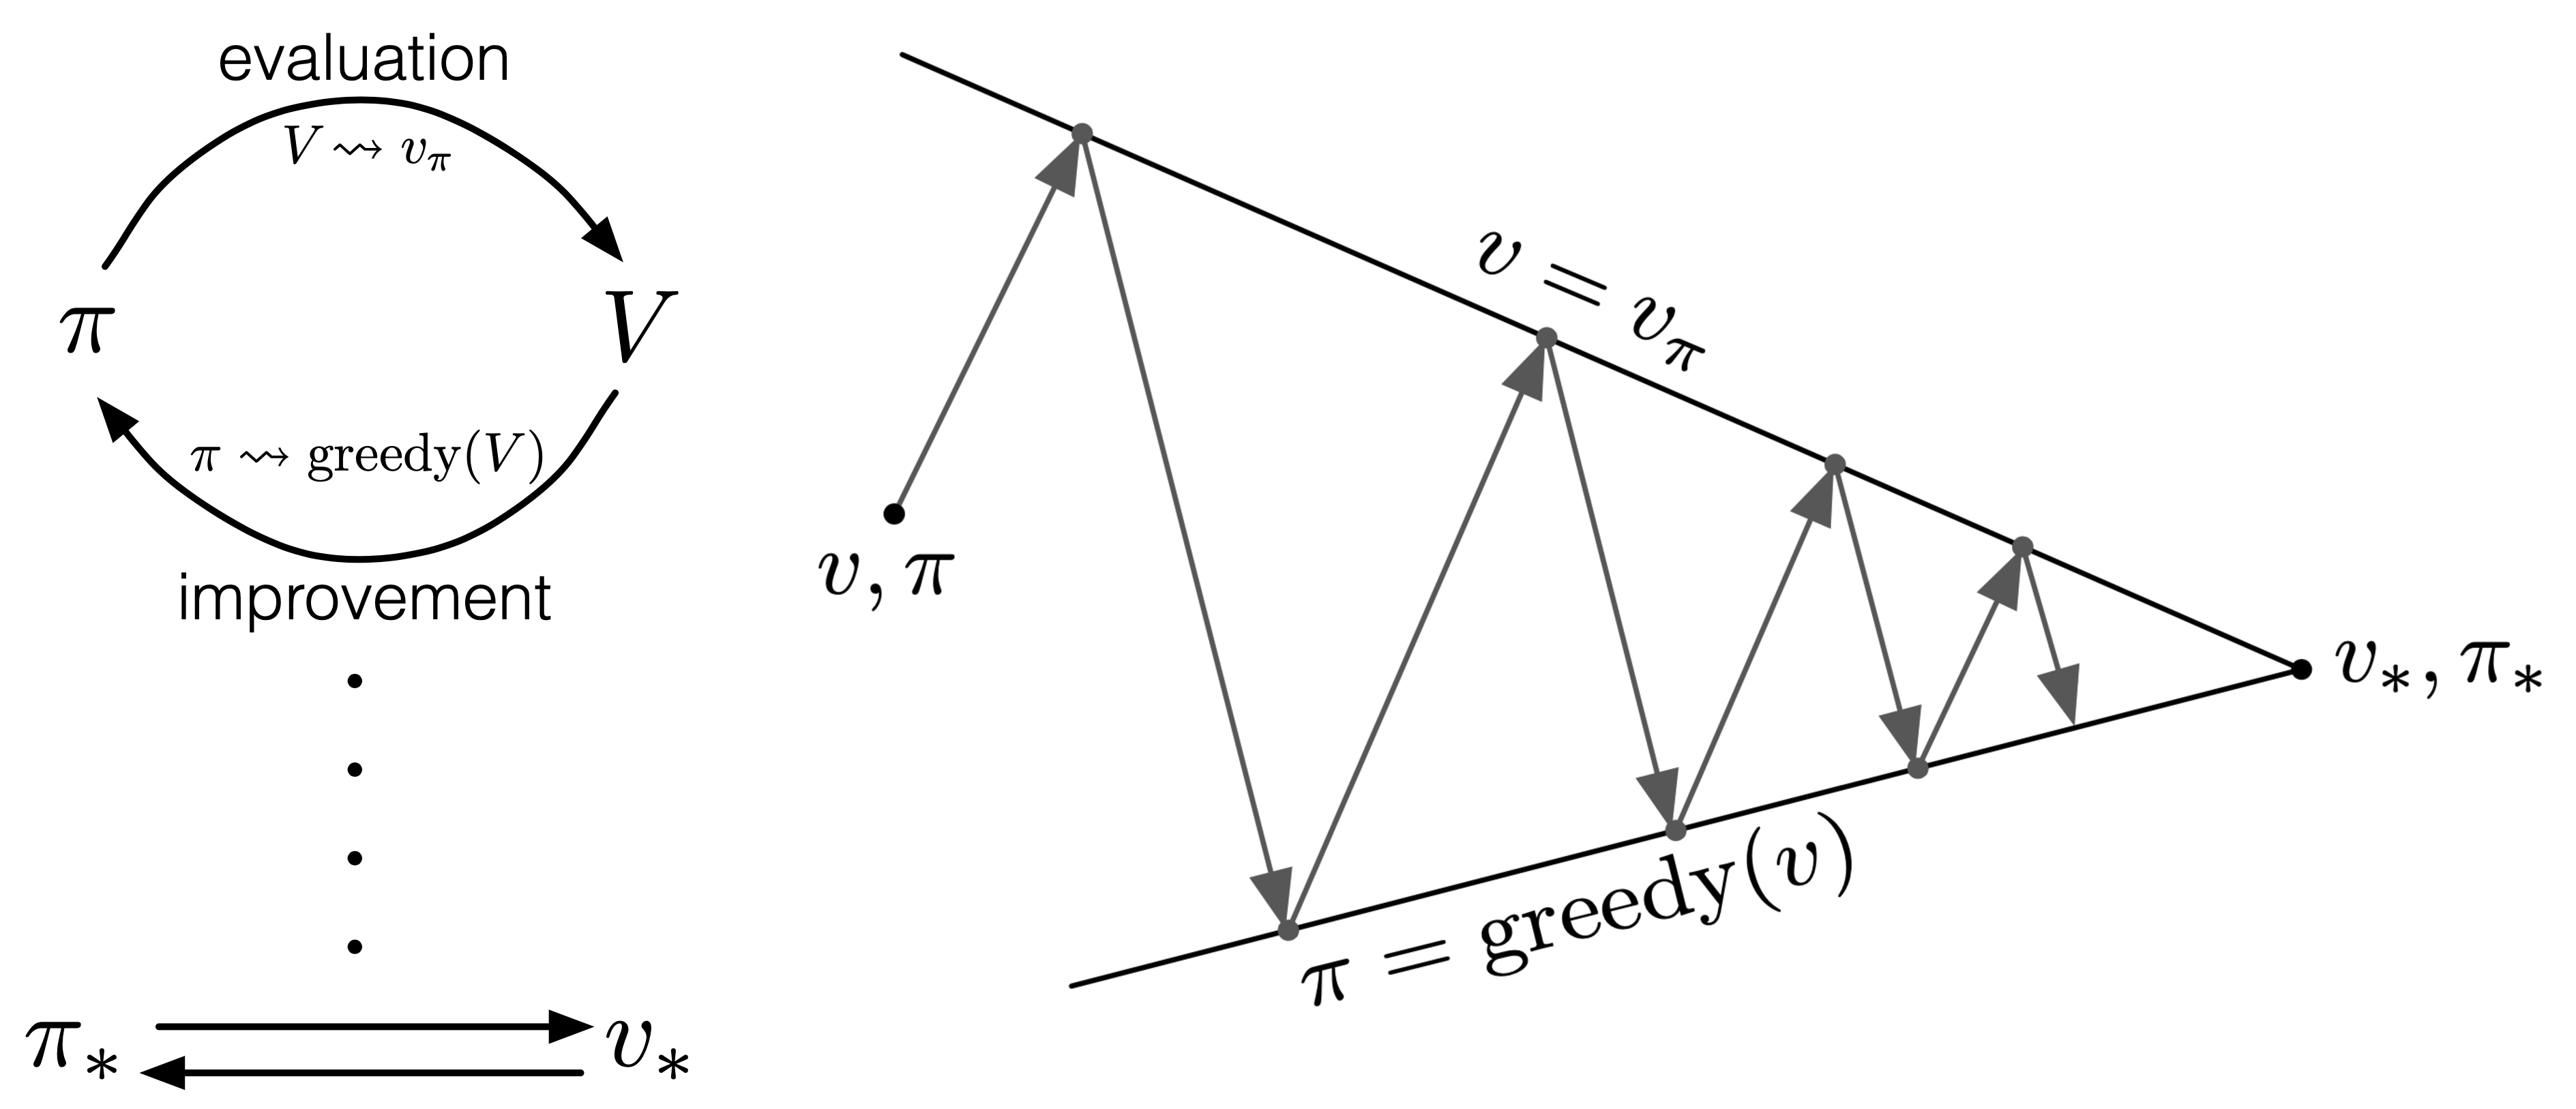
\includegraphics[width=0.7\textwidth]{images/gpi.jpg}
    \caption{GPI nach \cite[S.~86f]{Sutton1998}}
    \label{fig:GPI}
\end{figure}

Auf der anderen Seite kooperieren sich jedoch in dem Sinne, dass beide Prozesse sich nur dann Stabilisieren, wenn eine Strategie durch eine eigens evaluierte Nutzenfunktion gefunden worden ist, die zugleich gierig im Bezug auf genau diese ist, siehe Abb. \ref{fig:GPI}. Sie haben somit ein gemeinsames Ziel, die optimale Nutzenfunktion und die optimale Strategie zu finden.